
\chapter[Determinaci\'on del potencial h\'idrico]{Potencial h\'idrico}

\begin{huge}
	\begin{center}
		\textbf{Determinaci\'on del potencial h\'idrico en tejido con el m\'etodo gravim\'etrico}
	\end{center}
\end{huge}

\hspace{0.2cm}

\section{Introducci\'on}

% El agua en la planta
% Faltan citas 
El agua presenta un rol importante en la vida de la planta. Adem\'as, es considerada un nutriente porque es la forma en que las plantas absorben y asimilan los \'atomos de hidr\'ogeno durante la fotos\'intesis. Por otra parte, una de sus principales funciones es la de transporte, distribuci\'on de nutrientes, y metabolitos en la planta \citep{kirkham2014principles}. 

La principal magnitud que rige los movimientos del agua es el potencial qu\'imico ($\mu$), esto es la variaci\'on de energ\'ia libre ($\Delta G$) del agua en un punto a causa de los cambios en el volumen molar del agua. El potencial h\'idrico ($\Psi$) se deriva de el potencial qu\'imico, en otras palabras, $\Psi$ es la cantidad de trabajo que hay que proporcionar a una unidad de masa de agua vinculada a los tejidos de una planta, para transformarla a un estado de referencia como es el agua pura (con similar  presi\'on atmosf\'erica y temperatura) con su valor fijado en cero \citep{roger2001handbook}.

La conexi\'on entre $\mu$ y $\Psi$ es:

$$\Psi = \frac{\mu_w - \mu_w^{*}}{V} $$ 

Donde:

\begin{itemize}
	\item $\Psi = $ es el potencial h\'idrico y es expresado en unidades de presi\'on como pascal;
	\item  $\mu_w = $ el potencial qu\'imico del agua en el sistema bajo consideraci\'on;
	\item $\mu_w^{*} = $ potencial qu\'imico del agua pura a presi\'on atmosf\'erica y a la misma temperatura que el sistema en consideraci\'on;
	\item $V = $ volumen molar del agua (18 cm$^3$/mol), es decir, el volumen de un mol de agua.
\end{itemize}

Desde, $\Psi$ es una expresi\'on de estado de $\Delta G$ del agua, este es afectado por todos los factores en el cual cambian la $\Delta G$ o actividad qu\'imica de las mol\'eculas de agua. 

En consecuencia $\Psi$ es incrementado por: (1) desarrollo de presi\'on hidrost\'atica (turgencia); y (2) incremento de temperatura. $\Psi$ es disminuido por: (1) adici\'on de s\'olidos; (2) fuerzas m\'atricas que adsorben agua; (3) presi\'on negativa; y (4) reducci\'on de temperatura.

\subsection{Componentes del potencial h\'idrico}

El t\'ermino potencial h\'idrico fue propuesto por \citet{slatyer1960terminology}, en sus estudios de las relaciones planta-suelo-agua. 

En un sistema particular, el potencial h\'idrico puede ser expresado como la suma de cuatro componentes:

$$\Psi = \Psi_p + \Psi_s + \Psi_m + \Psi_g$$

Donde:

\begin{itemize}
	\item  $\Psi_p = $ potencial de presi\'on. Es el resultado de la presi\'on hidrost\'atica en la c\'elula, que ocurre cuando la presi\'on celular equilibra la diferencia de potencial hídrico entre el ambiente que rodea a la célula y el citoplasma;
	
	\item $\Psi_s = $ potencial osm\'otico. Es consecuencia a la presi\'on de solutos disueltos, disminuye la energ\'ia del agua y siempre es negativo;
	
	\item $\Psi_m = $ potencial m\'atrico. Es producto de fuerzas en las superficies de los s\'olidos. Su principal contribuci\'on es la fuerzas que retienen las mol\'eculas de agua por capilaridad, adsorci\'on e hidrataci\'on, en la superficie de las paredes celulares y el citoplasma;
	
	\item $\Psi_g = $ componente gravitacional. Es producto de la diferencia en energ\'ia potencial como resultado de la diferencia en altura con el nivel de referencia. Por lo general aumenta 0.01 MPa/m por encima del nivel del suelo. 
\end{itemize}

El potencial m\'atrico en las c\'elulas por lo general su efecto es muy peque\~no que puede ser ignorado, sin embargo, es particularmente importante en las primeras etapas de la absorción de agua por parte de las semillas secas (llamada imbibici\'on) y cuando se considera el agua retenida en los suelos \citep{hopkins2009introduction}. El componente gravitacional suele ser considerado cuando se mide el movimiento en los \'arboles. Por lo tanto, el potencial h\'idrico puede ser definido como: 

$$\Psi = \Psi_p + \Psi_s$$

En relaci\'on a la idea anterior, podemos replantear la fuerza motriz del movimiento de agua como el \textbf{gradiente del potencial h\'idrico} (Fig.~\ref{fig:gradiente}), en otras palabras, el agua se desplazar\'a de una regi\'on de $\Psi$ menos negativo hacia una regi\'on de $\Psi$ m\'as negativa. 

\begin{figure}[h]
	\begin{leftbar}
	
	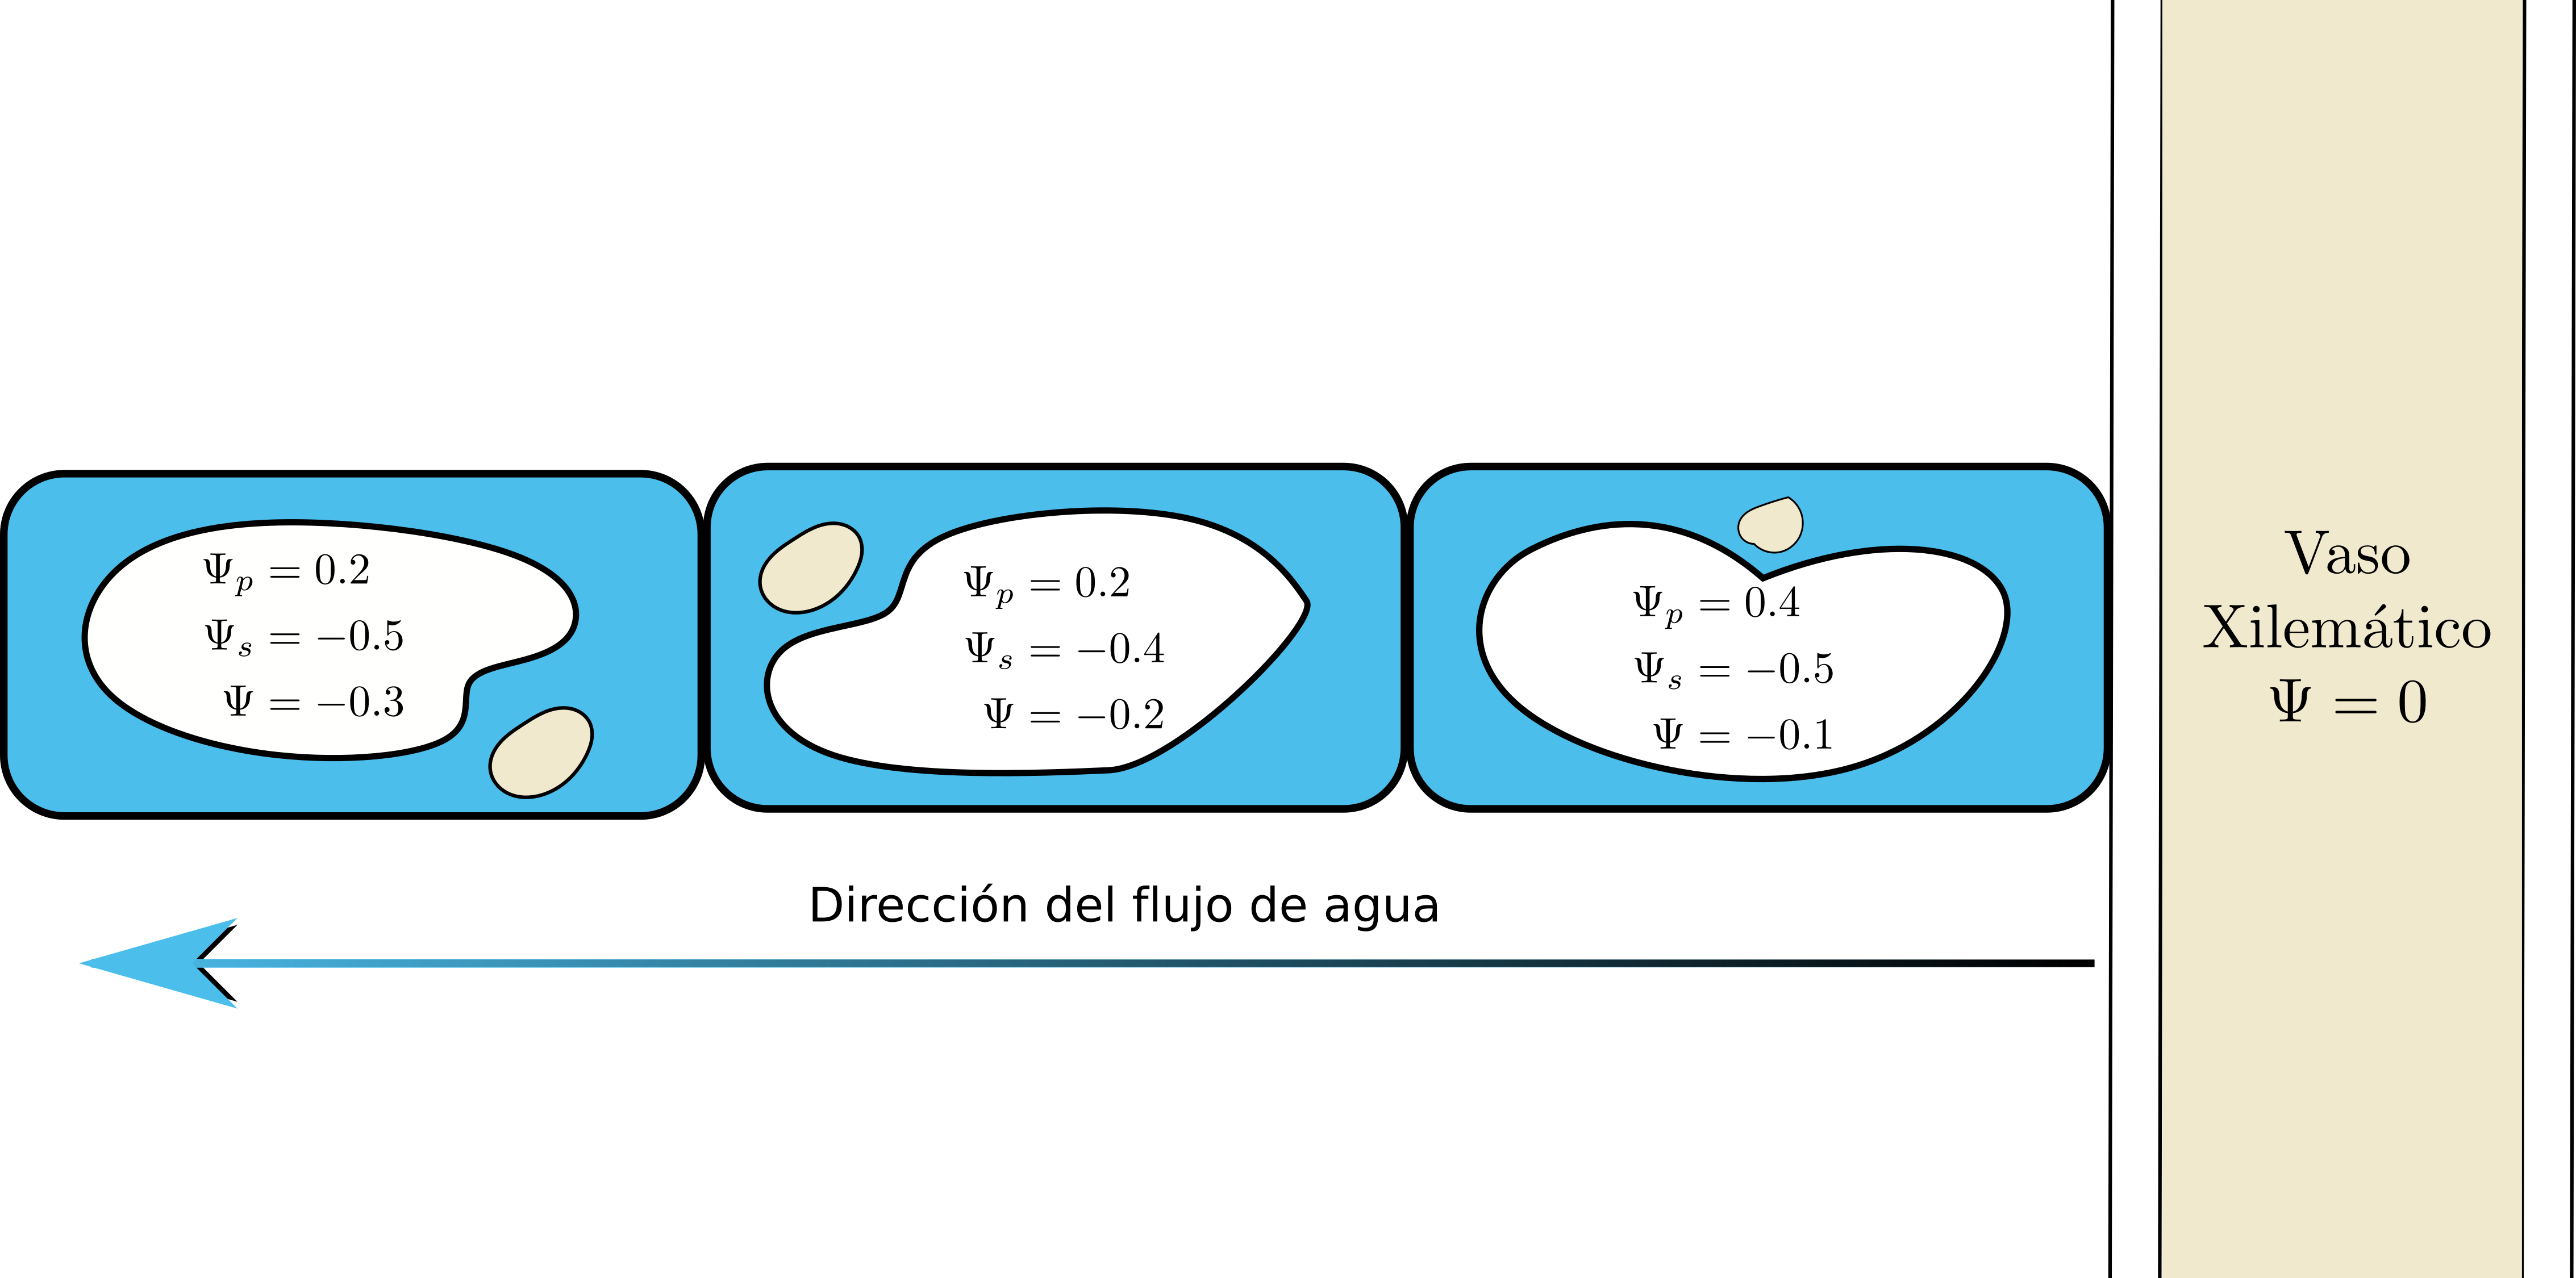
\includegraphics[width=\textwidth]{Gradiente_potencial}
	\centering
	\caption{\textit{Diagrama en el que se ilustran las contribuciones del potencial osmótico ($\Psi_s$), el potencial de presión ($\Psi_p$ ) y el potencial hídrico ($\Psi$) al movimiento del agua entre las células (Adaptado de \citealt{hopkins2009introduction}). Los valores de $\Psi$ se expresan en MPa.}}
	\label{fig:gradiente}
	
	\end{leftbar}
	
\end{figure}

La forma de calcular $\Psi_s$ para muchas soluciones biol\'ogicas es con la relaci\'on de van't Hoff:

$$ \Psi_s = -C i R T$$

Donde:

\begin{itemize}
	\item $C = $ concentraci\'on de soluto expresada en moles
	\item $i = $ constante de ionizaci\'on, para la sacarosa es igual a 1
	\item $R = $ constante de gases, su valor es 0.00831 Kg MPa/mol/K
	\item $T = $ Temperatura en grados Kelvin ($^\circ$C + 273) 
\end{itemize}

\subsection{Medici\'on del potencial h\'idrico}

El potencial h\'idrico para diferentes tejidos en plantas puede ser medido por los siguientes m\'etodos:

\begin{enumerate}
	\item Psicrom\'etrico de termopares
	\item M\'etodo de c\'amara de presi\'on
	\item M\'etodo gravim\'etrico 
	\item M\'etodo sonda de presi\'on
\end{enumerate}


\subsection{Principio}

Las c\'elulas vegetales ajustan constantemente su estado h\'idrico a consecuencia de los cambios en el contenido de agua del entorno y a variaciones del estado metab\'olico. Cuando una c\'elula se encuentra en un entorno isot\'onico, se puede decir que la c\'elula se encuentra en \textbf{plasm\'olisis incipiente} (Fig. ~\ref{fig:pasmolisis}) que dicha condici\'on el protoplasto apenas llena el volumen celular. En consecuencia, cuando una c\'elula se encuentra en dicho estado el $\Psi_p$ equivale a cero y el $\Psi$ de la c\'elula es igual al $\Psi_s$ \citep{NOBEL2020491}. Cabe considerar, por otra parte que si la c\'elula se encuentra en un soluci\'on hipot\'onica (agua destilada), es decir, una soluci\'on con menor contenido de solutos, debido a esto el agua entrar\'a a la c\'elula y provocar\'a un diluci\'on en el contenido vacuolar generando un mayor potencial de presi\'on. El agua dejar\'a de entrar a la c\'elula cuando el $\Psi_s$ y $\Psi_p$ se equilibren, en consecuencia el potencial h\'idrico equivale a cero ($\Psi = 0$). Por otra parte, cuando la c\'elula est\'a sumergida en una soluci\'on hipert\'onica, es decir, una soluci\'on con mayor cantidad de solutos; el gradiente del $\Psi$ favorece la p\'erdida de agua en la c\'elula. Dicha condici\'on se le conoce como plasm\'olisis generando que el protoplasto se separe de la pared celular. 

\begin{figure}[h]
	
	\begin{leftbar}
		
		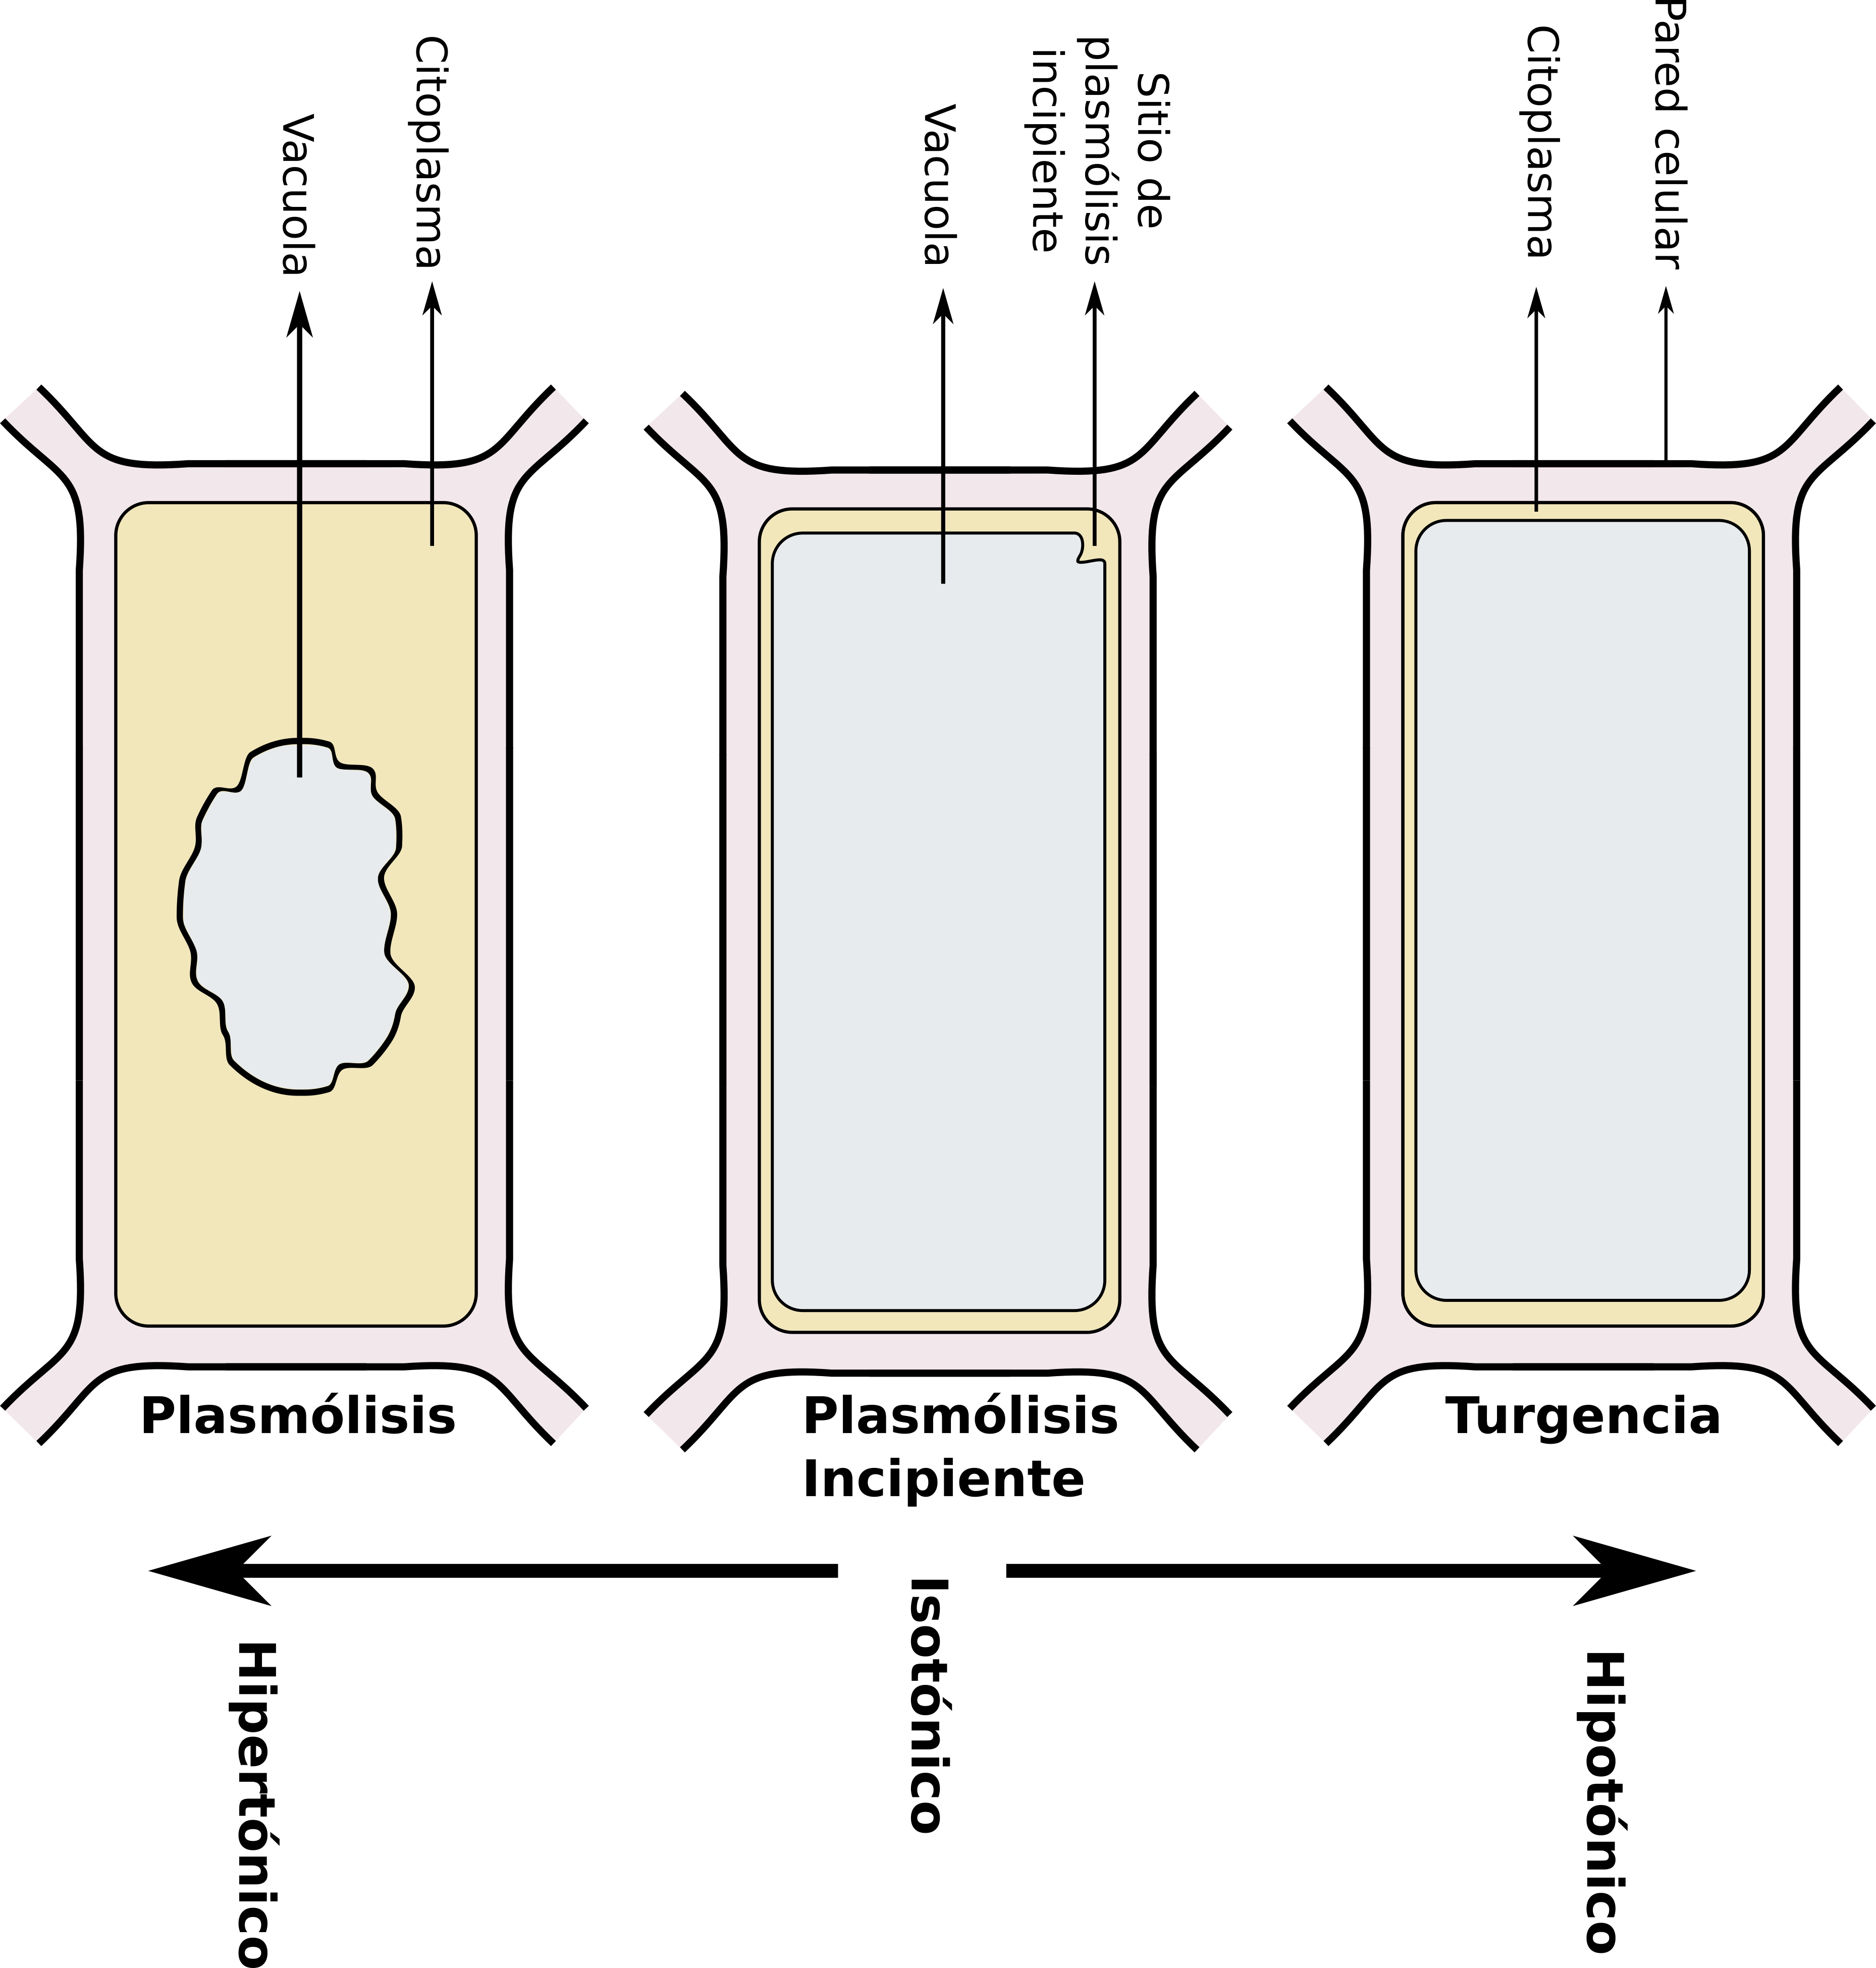
\includegraphics[width=\textwidth]{Plasmolisis}
		\centering
		\caption{\textit{Estado de la c\'elula cuando se encuentra en diferentes condiciones del medio extracelular.}}
		\label{fig:pasmolisis}
		
	\end{leftbar}

\end{figure}

De este modo cuando un tejido se sumerge en soluciones con potencial osm\'otico conocido estos cambiaran su peso, ya que el volumen celular cambia dependiendo de la concentraci\'on osm\'otica de la soluci\'on. Por lo tanto, en est\'a pr\'actica vamos a conocer el potencial osm\'otico de la papa \textit{Solanum tuberosum} para estimar el punto isosmotico.


\section{Objetivo general}

Determinar el potencial h\'idrico en papa \textit{Solanum tuberosum}.

\section{Objetivo espec\'ifico}

\begin{enumerate}
	
	\item Determinar el peso de los tejidos en papa \textit{Solanum tuberosum} con diferentes soluciones de sacarosa. 
	
	\item Evaluaci\'on del potencial h\'idrico en tejidos de papa \textit{Solanum tuberosum}.
	
\end{enumerate}

\section{Materiales}

\subsection{Material requerido}

\begin{enumerate}
	\item 10 tubos c\'onicos
	\item Nueve vasos de precipitados 
	\item Piceta de agua destilada
	\item Probeta de 100 mL
	\item Cinta adhesiva
	\item Agua destilada
	\item Sacarosa (masa molecular 342.3 g/mol)
	\item Azul de metileno
	\item Papa
	%\item Tub\'erculo de cebolla
\end{enumerate}

\subsection{Material por grupo}

\begin{enumerate}
	\item Balanza anal\'itica
	\item Papel secante
	\item Azul de metileno
\end{enumerate}

\section{Metodolog\'ia}

\subsection{Preparaci\'on de reactivos}

Necesitamos calcular la cantidad de sacarosa para preparar 100 mL de soluci\'on en las siguientes concentraciones molares \footnote{\footnotesize Una soluci\'on 1 molar (1 M) contiene el peso molecular de una sustancia (en gramos) por 1L de soluci\'on.} : \textbf{0.05, 0.1, 0.2, 0.25, 0.3, 0.4, 0.5, 0.7, 0.8 M}.

El peso molecular de la sacarosa es de 342.3 g/M. Por lo tanto, primero calculamos cu\'antos gramos se necesitan para obtener 1 L de soluci\'on a 0.05 M. 

\newpage

Lo resolvemos por una simple regla de tres:

$$\frac{342.3 \text{ g}}{1 \text{ M}} = \frac{\text{\textbf{\textit{x}}} \text{ g}}{0.05 \text{ M}}$$

Se obtiene:

$$ \text{\textbf{\textit{x}}} \text{ g} = \frac{342.3 \text{ g}}{1 \text{ M}} \times 0.05 \text{ M} = 17.12 \text{ g} $$

Por tanto, para preparar 1L de sacarosa a 0.05M, se requiere 17.12g sacarosa.

Establecemos una segunda regla de tres para calcular la cantidad de sacarosa necesaria para preparar 100 mL de un soluci\'on 0.05 M. 

$$\frac{17.12 \text{ g}}{1000 \text{ mL}} = \frac{\text{\textbf{\textit{x}}} \text{ g}}{100 \text{ mL}}$$

Resolviendo la expresi\'on:

$$ \text{\textbf{\textit{x}}} \text{ g} = \frac{17.12 \text{ g}}{1000 \text{ mL}} \times 100 \text{ mL} = 1.71 \text{ g} $$

Por lo tanto, para preparar 100 mL de una soluci\'on de sacarosa a 0.05 M, se necesita disolver 1.17 g de sacarosa en un volumen final de 100 mL de agua destilada.

Para las siguientes concentraciones los pesos estimados son:

\begin{tabular}{p{0.33\textwidth}p{0.33\textwidth}p{0.33\textwidth}}
 0.05 M = 1.71 g  &  0.25 M = 8.56 g & 0.5 M = 17.12 g \\
0.1 M = 3.42 g & 0.3 M = 10.27 g & 0.7 M = 23.96 g \\
 0.2 M = 6.85 g & 0.4 M = 13.69 g & 0.8 M = 27.38 g
\end{tabular}

\subsection{Procedimiento}

\begin{itemize}
	\item Tomar 10 secciones homog\'eneas de un tub\'erculo de papa (Ver la figura~\ref{fig:Diagrama_1}).
	\item Pesar cada secci\'on en la balanza anal\'itica (peso inicial).
	\item Introduzca una secci\'on por cada concentraci\'on de sacarosa y agregar una gota de azul de metileno. Dejar incubar por 45 minutos.
	\item Despu\'es del tiempo de incubaci\'on, remover las secciones y secar el exceso de soluci\'on con papel absorbente.
	\item Pesar las secciones de papa en el orden que fueron colocadas.
	\item Anotar los datos en el cuadro~\ref{resultados:potencial} y calcular el porcentaje de cambio en peso de cada muestra. 
\end{itemize}

\begin{figure}[h]
	
	\begin{leftbar}
	
	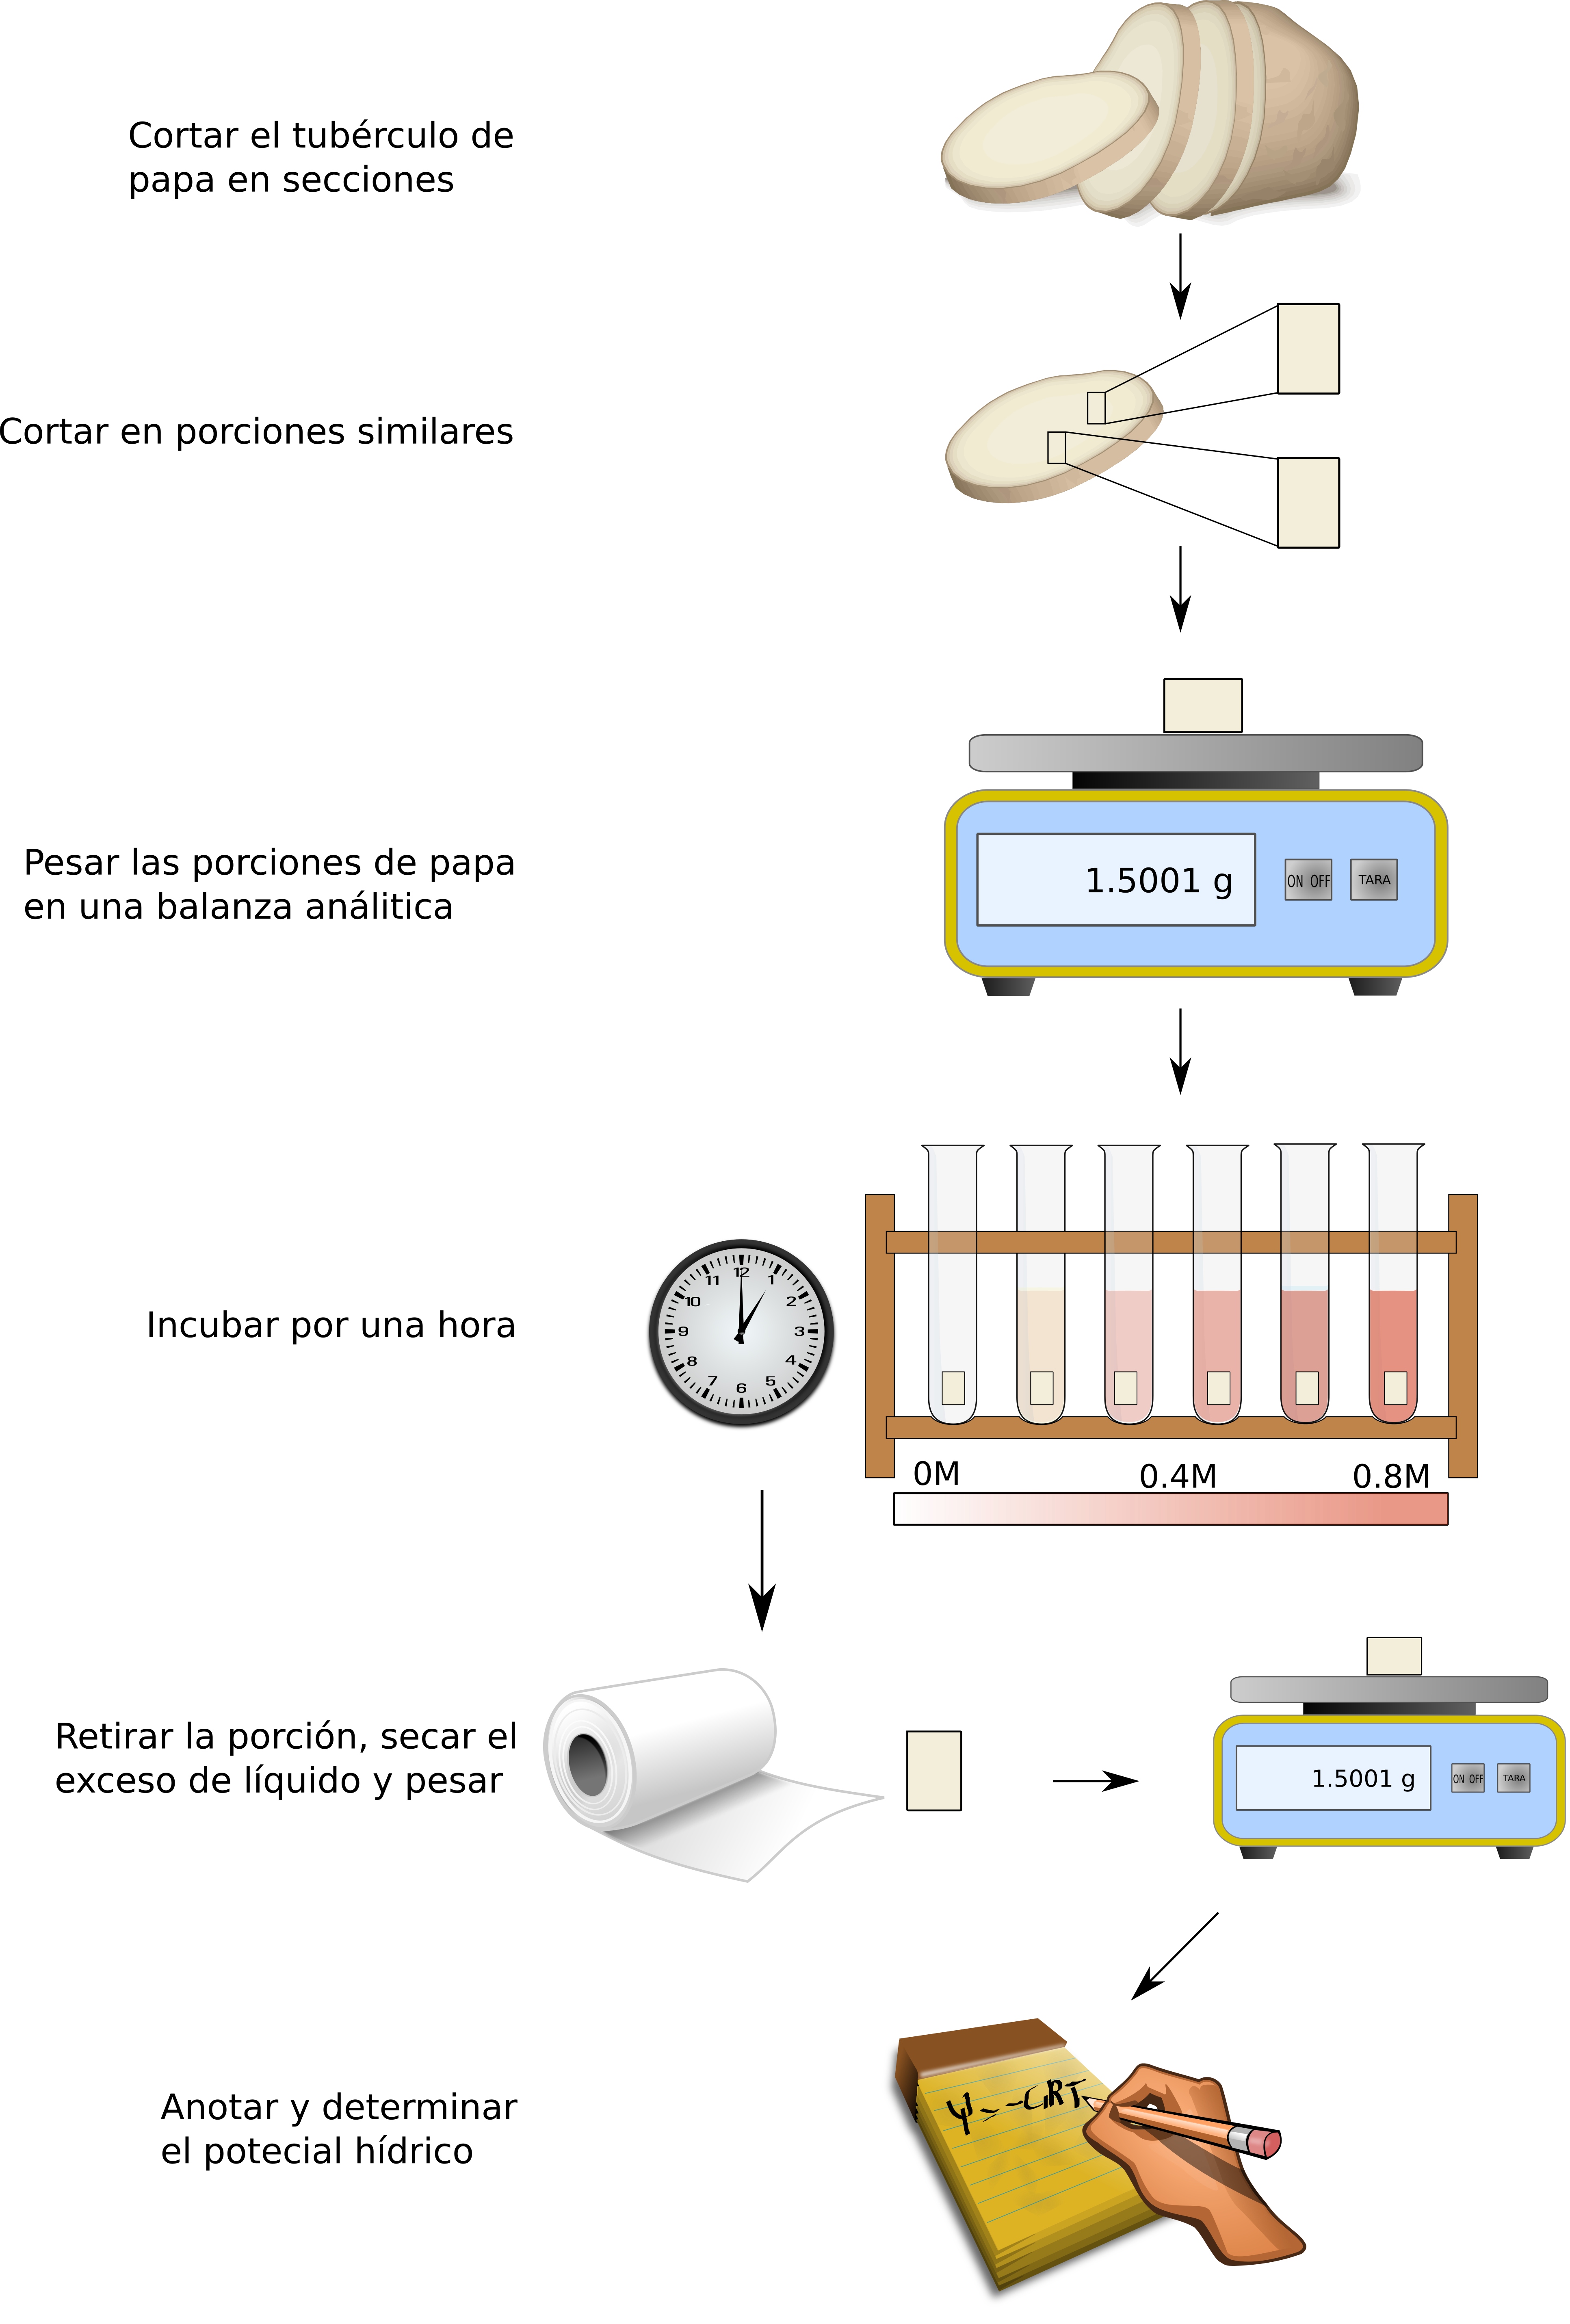
\includegraphics[width=\textwidth]{diagrama.png}
	\centering
	\caption{\textit{Diagrama de procedimientos para el m\'etodo volumen/peso para la determinaci\'on del potencial h\'idrico en tejido de papa.}}
	\label{fig:Diagrama_1}
	
	\end{leftbar}
	
\end{figure}

\section{Resultados}

\begin{table}[h!]
	\caption{Datos de cambio de peso en porciones de papa incubadas en diferentes soluciones de sacarosa.}
	
	\label{resultados:potencial}
	\centering
	\begin{tabular}{|p{0.17\textwidth}|p{0.17\textwidth}|p{0.17\textwidth}|p{0.17\textwidth}|p{0.17\textwidth}|}
	
	\hline  &&&& \\
	Soluci\'on sacarosa (M) & Peso inicial (g) & Peso final (g) & $\Delta$ peso$^\dagger$ (g) & Porcentaje $\Delta$ peso$^\mp$ \\
	&&&& \\
	\hline 
	0.00 &&&& \\
	0.05 &&&& \\
	0.10 &&&& \\
	0.20 &&&& \\
	0.25 &&&& \\
	0.30 &&&& \\
	0.40 &&&& \\
	0.50 &&&& \\
	0.70 &&&& \\
	0.80 &&&& \\

	\hline 

	\multicolumn{5}{l}{\footnotesize $^\dagger$ $\Delta$ peso = Peso final - Peso inicial. } \\
	\multicolumn{5}{l}{\footnotesize $^\mp$ Porcentaje $\Delta$ peso = $\Delta$ peso / Peso inicial $\times$ 100 }	
	
	\end{tabular}
\end{table}

\begin{itemize}
	\item Elaborar un gr\'afico (fig.~\ref{fig:ejem_concentracion}) del porcentaje de cambio en peso del tejido en funci\'on de la concentraci\'on de sacarosa (M).
	\item Determinar la concentraci\'on de sacarosa en la cual no se presento un cambio en el peso del tejido.
	\item Calcular el $\Psi_s$ de la soluci\'on con la ecuaci\'on de van't Hoff. 
\end{itemize}

\begin{figure}[h!]
	
	\begin{leftbar}
		
		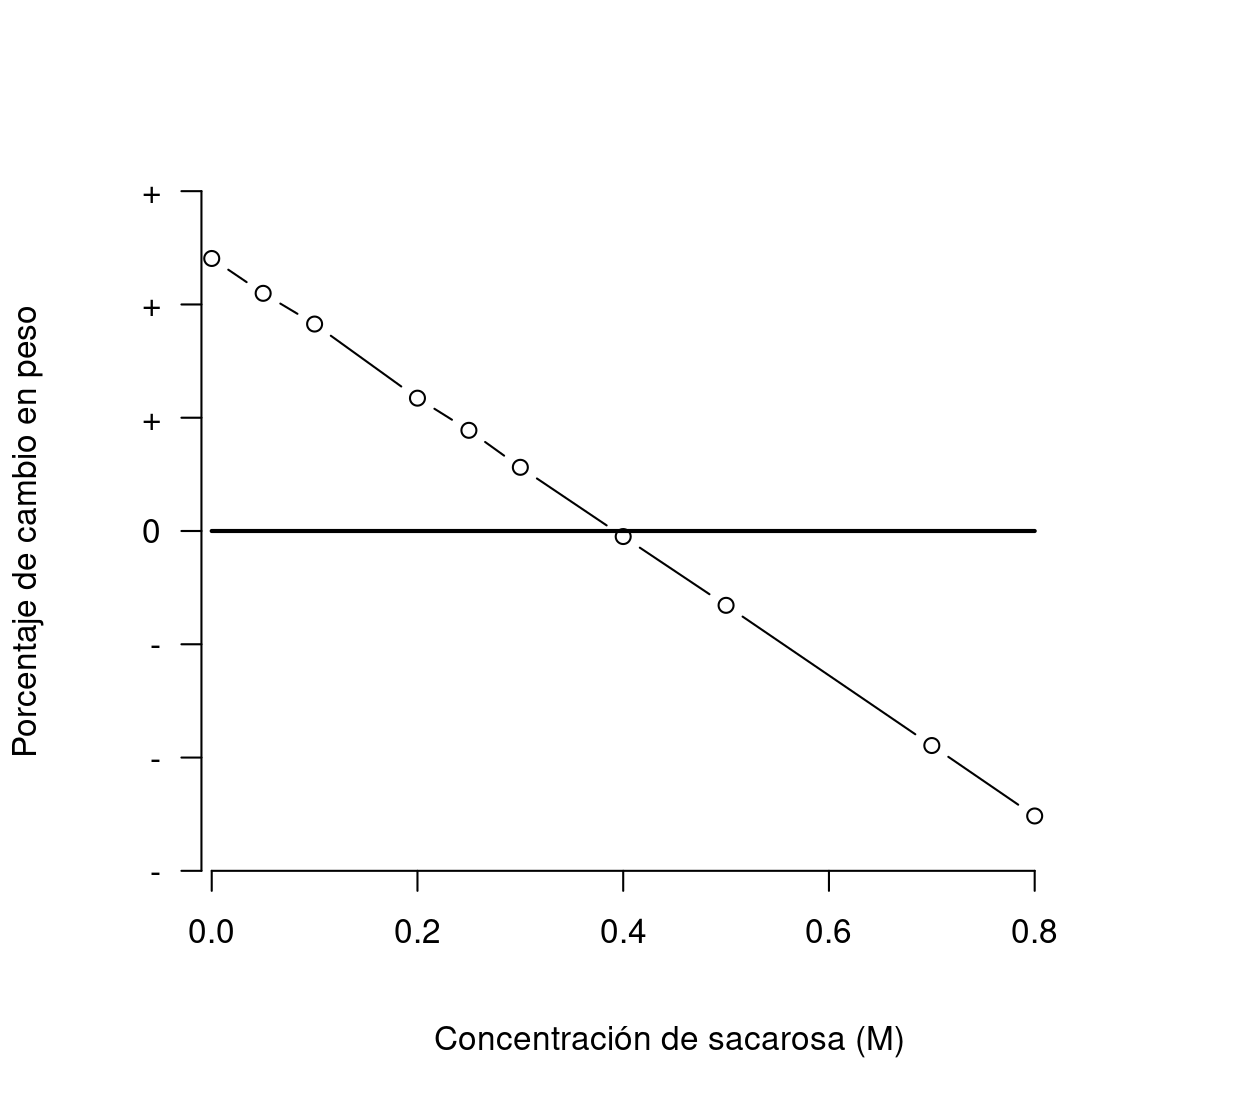
\includegraphics[width=\textwidth]{graf_cambio}
		\centering
		\caption{\textit{Representaci\'on del cambio en peso en funci\'on de la concentraci\'on de sacarosa.}}
		\label{fig:ejem_concentracion}
		
	\end{leftbar}
	
\end{figure}


\section{Cuestionario}

\begin{enumerate}
	\item \textquestiondown De que forma el concepto de potencial h\'idrico ayuda a explicar los movimientos de agua en los tejidos vegetales?
	\item Cuando una c\'elula est\'a totalmente turgente, \textquestiondown cu\'al de las siguientes opciones equivale a cero?
		\begin{itemize}
			\item Potencial osm\'otico
			\item Potencial h\'idrico
			\item Presi\'on de turgencia
		\end{itemize}
	%\item Utilizando un corte delgado en la epidermis de una cebolla, se obtiene los siguientes datos; presenta un intercambio nulo con una soluci\'on de $ClNa$ 0.150 M a 25 $^\circ$C; la plasm\'olisis incipiente se presenta en una soluci\'on de $ClNa$ 0.293 M a la misma temperatura. Determine los distintos componentes del potencial h\'idrico de las c\'elulas en la epidermis de cebolla en el estado inicial y final del la plam\'olisis. Considerando que $\Psi_m$ es casi nulo y las membranas no son permeables al $ClNa$. 
\end{enumerate}

